\section{Internals}
\label{sec:internals}
The tool \Tool relies on the Python packages
\begin{itemize}[itemsep=0pt]
	\item \Code{toro}
	\item \Code{pycpa}
\end{itemize}
and the main script
\begin{itemize}[itemsep=0pt]
	\item \Code{toro\_main.py}
\end{itemize}
Details about the \Code{pycpa} package can be found in the online documentation at \url{https://pycpa.readthedocs.io}.
The other two components are discussed in more detail in the following sections \ref{sec:script} and \ref{sec:toro_lib}.
    
\subsection{User Script}
\label{sec:script}
The main script \Code{toro\_main.py} consists of two methods (cf. Figure \ref{fig:toro_internals}):

\paragraph{get\_system\_dirs(dir)}
The script \Code{toro\_main.py} starts with the main method and passes the call parameter (folder path) to the \Code{get\_system\_dirs(dir)} method. \\
The method \Code{get\_system\_dirs(dir)} searches for existing systems under the specified path. 
If more than one system is found, the user can choose from a list which systems should to be analyzed. 

\paragraph{perform\_analysis(dir)}
The method \Code{perform\_analysis(dir)} 
\begin{itemize}[itemsep=0pt]
	\item starts a user query to identify the type of system and verify assumptions about the system,
	\item parses the csv-files which specify the system,
	\item calculates the maximum end-to-end latencies and robustness margins,
	\item generates of diagrams,
	\item logs the numerical results (\Code{RESULTS\_LOG.txt}), 
\end{itemize}
for each of the selected systems.
 %
\begin{figure}[H]
		\centering
		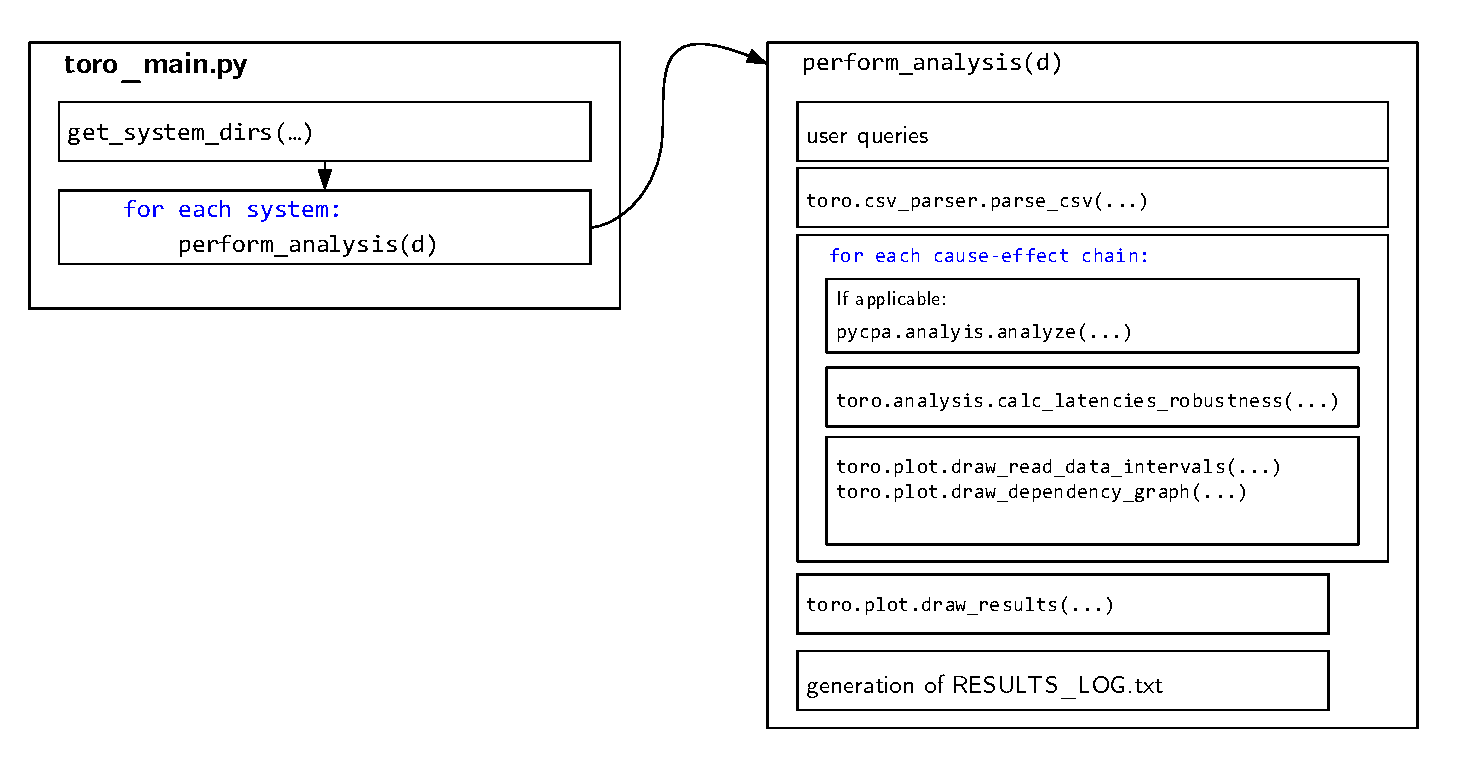
\includegraphics[width=\textwidth]{fig/toro_architecture.pdf}
		\caption{Internals of the main script \Code{toro\_main.py}}
		\label{fig:toro_internals}
\end{figure}

 
\subsection{Toro Package}
\label{sec:toro_lib}
    
This section describes the modules in the package \Code{toro}.

\paragraph{toro.model}
This module defines the data structures required within the software. 
It is an extension of the module of the same name from the \Code{pycpa} package.

\paragraph{toro.analysis}
This module contains the \Code{calc\_latencies\_robustness} class.
When an object of this class is initialized and a chain is passed as an argument, then the maximum latency and the robustness margins for each task are computed.

\paragraph{toro.csv\_parser}
This module reads the CSV-files from the specified folder and transfers them into the software's internal data structure. 
If files are not available or data is not properly defined, an error message is issued. 
The parser is called via the \Code{prase\_csv} class, which requires the folder path of the system to be analyzed as argument.

\paragraph{toro.plot}
The module plots creates graphical representations of the analysis results; the three different types of graphs have been discussed in the section \ref{sec:outputs}.
The module consists of several classes, each is designed for one of the graphical output formats. 

\begin{description}
\item[\Code{image}] 
The \Code{image} class provides the basic functions to draw circles, lines, text and other elements in an SVG image.  
%
\item[\Code{draw\_read\_data\_intervals}] 
This class draws the read and data intervals of jobs in a representative time window on the basis of the analysis results. 
In addition, the computed properties -- maxmimum end-to-end latency and the robustness margins for the isolated chain -- can be drawn using the options "all", "none", "first" and "last". 
A further option is to include the "Dependency Polygon":
\begin{itemize}
		\item max\_data\_age = all | first | last | none
		\item robustness\_margin = all | first | last | none
		\item dependency\_polygon = True | False.
\end{itemize}    
												
\item[\Code{draw\_dependency\_graph}] 
The reachability graph illustrates possible instances of a cause-effect chain. As the call parameter are the analysis results required.
%
\item[\Code{draw\_results}] 
The relevant results of all tasks and cause-effect chains of a system are displayed in an overview graph. 
Chains and tasks are used as call parameters. 
%
\end{description}